
\documentclass[10pt]{exam}
\usepackage{graphicx}
\usepackage{listings}

\newcommand{\R}{\mathbb{R}}
\newcommand{\changes}[1]{{\color{red} #1}}
\usepackage{xcolor}
\usepackage[english]{babel}
\usepackage{amsmath,amssymb,amsthm,mathdots}
\usepackage{graphicx}
\usepackage[colorinlistoftodos]{todonotes}


\renewcommand{\thequestion}{\arabic{question} }
\renewcommand\questionlabel{\llap{\thequestion)}}


\usepackage{xcolor}
\definecolor{SolutionColor}{rgb}{0.1,0.3,1}

\unframedsolutions
\shadedsolutions
\definecolor{SolutionColor}{rgb}{0.9,0.9,1}
\renewcommand{\solutiontitle}{\textbf{Solution}$:\>$  }




%Mathcal and 
\newcommand{\mb}[1]{\mathbb{#1}}
\newcommand{\mc}[1]{\mathcal{#1}}

%Various possibilities for norms
\newcommand{\norm}[2]{\|#1\|_{#2}}
\newcommand{\normtwo}[1]{\|#1\|_{2}}
\newcommand{\normp}[1]{\|#1\|_{p}}

\newcommand{\rn}{\mathbb{R}^n}
\newcommand{\rnn}{\mathbb{R}^{n\times n}}
\newcommand{\rmn}{\mathbb{R}^{m\times n}}



%Boldface for vectors and tildes
\renewcommand{\vec}[1]{{#1}•}
\newcommand{\mat}[1]{{#1}•}

\newcommand{\vect}[1]{\widetilde{\boldsymbol{#1}}}
\newcommand{\matt}[1]{\widetilde{\boldsymbol{#1}}}

%Column and row equivalence
\newcommand{\roweq}{\stackrel{\text{row}}{\sim}}
\newcommand{\coleq}{\stackrel{\text{col}}{\sim}}

\newtheorem{definition}{Definition}
\newtheorem{example}{Example}
\newtheorem{fact}{Fact}
\newtheorem{remark}{Remark}


%Vector spaces
\newcommand{\rank}{\text{rank}\,}
\renewcommand{\dim}{\text{dim}\,}
\newcommand{\Span}[1]{\text{Span}\,\{#1\}}
\newcommand{\basis}[1]{\left\{ #1\right\}}


%Matrix environments
\newcommand{\bmat}[1]{\begin{bmatrix}#1\end{bmatrix}}
\newcommand{\pmat}[1]{\begin{pmatrix}#1\end{pmatrix}}
\newenvironment{amatrix}[1]{%
  \left(\begin{array}{@{}*{#1}{c}|c@{}}
}{%
  \end{array}\right)
}


%Trace and determinant
\newcommand{\diag}{\mathsf{diag}\,}
\newcommand{\range}{\mathsf{range}\,}
\newcommand{\trace}{\mathsf{trace}\,}


\usepackage{hyperref}
\title{MA 402: Project 2}
\author{Richard Watson, Mountain Chan, Cole Nash}
%\date{}
\begin{document}
\maketitle
\textbf{Instructions}: 

\begin{itemize}
\item Detailed instructions regarding submission are available on the class website\footnote{\url{https://github.ncsu.edu/asaibab/ma402/blob/master/project.md}}.
\item The zip file should contain five files hw2.pdf, hw2.tex, classnotes.sty, swift.mat, and deblur.mat. 

\item More instructions:
\begin{itemize}
\item MATLAB users: use \verb|loadmat| (type \verb|who| to display what variables are in your workspace. 
\item Python users: use \verb|scipy.io.loadmat|. This will return a dictionary with all the necessary variables.
\end{itemize}
\item For plotting, you may consider using \verb|imshow|.
\end{itemize}

\vspace{2mm}


\section{Pen-and-paper exercises}
The problems from this section total $20$ points.
\begin{questions}
\question [10] Consider the matrix $A$ with the SVD
\[ A = \bmat{ 4 & 0\\ -5 & -3 \\ 2 & 6} = U \bmat{6 \sqrt{2}   &  0 \\ 0 & 3\sqrt{2}  \\ 0 & 0} V^\top , \]
where
\[ U   = \frac13\bmat{ 1  & -2 &  2 \\ -2  & 1 & 2\\  2 & 2 & 1} \qquad V = \frac{1}{\sqrt{2}} \bmat{1 & -1 \\ 1  & 1}.  \]
\begin{parts}
\part [0] Verify for yourself that it is indeed the SVD of $A$, and that $U,V$ are orthogonal. 

$A = U \Sigma V^T$ :
\begin{align*}
    A &= \frac{1}{3} \bmat{ 1  & -2 &  2 \\ -2  & 1 & 2\\  2 & 2 & 1} \bmat{6 \sqrt{2}   &  0 \\ 0 & 3\sqrt{2} \\ 0 & 0} \frac{1}{\sqrt{2}} \bmat{1 & 1 \\ -1  & 1}\\
    &= \frac{3\sqrt{2}}{3\sqrt{2}} \bmat{ 1  & -2 &  2 \\ -2  & 1 & 2\\  2 & 2 & 1} \bmat{2   &  0 \\ 0 & 1 \\ 0 & 0} \bmat{1 & 1 \\ -1  & 1} \\
    &= \bmat{2 & -2 \\ -4 & 1 \\ 4 & 2} \bmat{1 & 1 \\ -1 & 1} \\
    &= \bmat{4 & 0 \\ -5 & -3 \\ 2 & 6} = A
\end{align*}

$UU^T = U^TU$ :
\begin{align*}
    U &= \frac13 \bmat{1 & -2 & 2 \\ -2 & 1 & 2 \\ 2 & 2 & 1}\\
    U^T &= \frac13 \bmat{1 & -2 & 2 \\ -2 & 1 & 2 \\ 2 & 2 & 1}\\
    UU^T &= \frac{1}{9} \bmat{1 & -2 & 2 \\ -2 & 1 & 2 \\ 2 & 2 & 1} \bmat{1 & -2 & 2 \\ -2 & 1 & 2 \\ 2 & 2 & 1} = \frac{1}{9} \bmat{9 & 0 & 0 \\ 0 & 9 & 0 \\ 0 & 0 & 9} = \bmat{1 & 0 & 0 \\ 0 & 1 & 0 \\ 0 & 0 & 1} = I\\
    U^TU &= \frac{1}{9} \bmat{1 & -2 & 2 \\ -2 & 1 & 2 \\ 2 & 2 & 1} \bmat{1 & -2 & 2 \\ -2 & 1 & 2 \\ 2 & 2 & 1} = \frac{1}{9} \bmat{9 & 0 & 0 \\ 0 & 9 & 0 \\ 0 & 0 & 9} = \bmat{1 & 0 & 0 \\ 0 & 1 & 0 \\ 0 & 0 & 1} = I
\end{align*}

$VV^T = V^TV$ :
\begin{align*}
    V &= \frac{1}{\sqrt{2}} \bmat{1 & -1 \\ 1 & 1}\\
    V^T &= \frac{1}{\sqrt{2}} \bmat{1 & 1 \\ -1 & 1}\\
    VV^T &= \frac{1}{2} \bmat{1 & -1 \\ 1 & 1}\bmat{1 & 1 \\ -1 & 1} = \frac{1}{2} \bmat{2 & 0 \\ 0 & 2} = \bmat{1 & 0 \\ 0 & 1} = I\\
    V^TV &= \frac{1}{2} \bmat{1 & 1 \\ -1 & 1}\bmat{1 & -1 \\ 1 & 1} = \frac{1}{2} \bmat{2 & 0 \\ 0 & 2} = \bmat{1 & 0 \\ 0 & 1} = I
\end{align*}

\part [1] What is the rank of this matrix? 

Rank is the number of singular values, so the rank of A is 2.

\part [2] From the full SVD of $A$, write down the thin SVD of $A$. 
\begin{align*}
    A &= \frac{1}{3} \bmat{1 & -2 \\ -2 & 1 \\ 2 & 2} \bmat{6\sqrt{2} & 0 \\ 0 & 3\sqrt{2}} \frac{1}{\sqrt{2}} \bmat{1 & 1 \\ -1 & 1}\\
    &= \bmat{1 & -2 \\ -2 & 1 \\ 2 & 2} \bmat{2 & 0 \\ 0 & 1} {\sqrt{2}} \bmat{1 & 1 \\ -1 & 1}\\
    &= \bmat{2 & -2 \\ -4 & 1 \\ 4 & 2} \bmat{1 & 1 \\ -1 & 1}\\
    &= \bmat{4 & 0 \\ -5 & -3 \\ 2 & 6} = A
\end{align*}

\part [3] Compute the best rank-$1$ approximation of $A$. 

\begin{align*}
    A_1 &= \frac{1}{3} \bmat{1 \\ -2 \\ 2} 6\sqrt{2} \frac{1}{\sqrt{2}} \bmat{1 & 1}\\
    &= \bmat{1 \\ -2 \\ 2} \bmat{1 & 1} = \bmat{2 & 2 \\ -4 & -4 \\ 4 & 4}
\end{align*}

\part [2] Compute the $2$-norm and the Frobenius norms of $A$.

2-norm :

\begin{align*}
    ||A||_2 = 6\sqrt{2} = 8.48528
\end{align*}

Frobenius norm :

\begin{align*}
    ||A||_F &= \big( (6\sqrt{2})^2 + (3\sqrt{2})^2\big) ^{\frac{1}{2}}\\
    &= (64 + 18)^{\frac{1}{2}} = \sqrt{82} = 9.05539
\end{align*}

\part [2] Using the SVD of $A$, write down the SVD of $A^\top$ and $A^\top A$. 

\begin{align*}
    A^T &= (U \Sigma V^T)^T\\
    &= V \Sigma ^T U^T\\
    &= \frac{1}{\sqrt{2}} \bmat{1 & -1 \\ 1 & 1} \bmat{6\sqrt{2} & 0 & 0 \\ 0 & 3\sqrt{2} & 0} \frac{1}{3} \bmat{1 & -2 & 2 \\ -2 & 1 & 2 \\ 2 & 2 & 1}\\
    &= \bmat{1 & -1 \\ 1 & 1} \bmat{2 & 0 & 0 \\ 0 & 1 & 0} \bmat{1 & -2 & 2 \\ -2 & 1 & 2 \\ 2 & 2 & 1}\\
    &= \bmat{2 & -1 & 0 \\ 2 & -1 & 0} \bmat{1 & -2 & 2 \\ -2 & 1 & 2 \\ 2 & 2 & 1}\\
    &= \bmat{4 & -5 & 2 \\ 0 & -3 & 6}
\end{align*}

\begin{align*}
    A^TA &= (U \Sigma V^T)^T(U \Sigma V^T)\\
    &= (V \Sigma ^T U^T)(U \Sigma V^T)\\
    &= V \Sigma ^2 V^T\\
    &= \frac{1}{\sqrt{2}} \bmat{1 & -1 \\ 1 & 1} \bmat{6\sqrt{2} & 0 \\ 0 & 3\sqrt{2}} \bmat{6\sqrt{2} & 0 \\ 0 & 3\sqrt{2}} \frac{1}{\sqrt{2}} \bmat{1 & 1 \\ -1 & 1}\\
    &= \bmat{1 & -1 \\ 1 & 1} \bmat{6 & 0 \\ 0 & 3} \bmat{6 & 0 \\ 0 & 3} \bmat{1 & 1 \\ -1 & 1}\\
    &= \bmat{6 & -3 \\ 6 & 3} \bmat{6 & 0 \\ 0 & 3} \bmat{1 & 1 \\ -1 & 1}\\
    &= \bmat{36 & -9 \\ 36 & 9} \bmat{1 & 1 \\ -1 & 1}\\
    &= \bmat{45 & 27 \\ 27 & 45}
\end{align*}

\end{parts}

\pagebreak

\question [10] Let $A \in \rmn. $ Recall: by definition, the Frobenius norm of $A$ is $\|A\|_F = \left( \sum_i\sum_j |a_{ij}|^2 \right)^{1/2}$. In this problem, we will derive the formula $$\|A\|_F=  \left(\sigma_1^2 + \dots + \sigma_r^2 \right)^{1/2}. $$ 
\begin{parts}
\part  The trace of a square matrix is the sum of its diagonals entries. Show (an alternative representation for the Frobenius norm): 

\[ \|A\|_F = \left( \trace(A^\top A) \right)^{1/2}. \]

\begin{align*}
    A &= \bmat{\vdots & & \vdots \\ v_1 & \cdots & v_n \\ \vdots & & \vdots}\\
    A^T &= \bmat{\cdots & v_1 & \cdots \\ & \vdots & \\ \cdots & v_n & \cdots}\\
    A^TA &= \bmat{v_1 \cdot v_1 & & \\ & \ddots & \\ & & v_n \cdot v_n} = \bmat{a_{11}^2 + \dots + a_{n1}^2 & & \\ & \ddots & \\ & & a_{n1}^2 + \dots + a_{nn}^2}\\
    \text{trace}(A^TA) &= (a_{11}^2 + \dots + a_{n1}^2) + \dots + (a_{n1}^2 + \dots + a_{nn}^2) = \sum_i^n \sum_j^n a_{ij}^2 = ||A||_F^2\\
    ||A||_F &= \big( \text{trace}(A^TA) \big)^\frac{1}{2}
\end{align*}

\pagebreak

\part Let $C,D$ be $n\times n$ square matrices. Show: $\trace(CD)  = \trace(DC)$. \\
{\em Remark}:  This is known as the cyclic property of trace, which is true despite the fact that in general $CD\neq DC$. A consequence of the cyclic property is: if $E$ has the same size as $C,D$, it implies 
\[ \trace(CDE) = \trace(DEC) = \trace(ECD). \]

\begin{align*}
    C &= \bmat{c_{11} & \cdots & c_{1n} \\ \vdots & \ddots & \vdots \\ c_{n1} & \cdots & c_{nn}}\\
    D &= \bmat{d_{11} & \cdots & d_{1n} \\ \vdots & \ddots & \vdots \\ d_{n1} & \cdots & d_{nn}}\\
    CD &= \bmat{c_{11}d_{11} + \dots + c_{1n}d_{1n} & & \\ & \ddots & \\ & & c_{n1}d_{n1} + \dots + c_{nn}d_{nn}} \\
    \text{trace}(CD) &= \sum_i^n \sum_j^n c_{ij}d_{ij}\\
    DC &= \bmat{d_{11}c_{11} + \dots + d_{1n}c_{1n} & & \\ & \ddots & \\ & & d_{n1}c_{n1} + \dots + d_{nn}c_{nn}} \\
    \text{trace}(DC) &= \sum_j^n \sum_i^n d_{ji}c_{ji}\\
    & \text{trace}(CD) = \text{trace}(DC)
\end{align*}

\part Using parts (a-c) complete the proof to show  $\|A\|_F =  \left(\sigma_1^2 + \dots + \sigma_r^2 \right)^{1/2}$.
 
\begin{align*}
    \text{trace}(A^TA) &= \text{trace}(V\Sigma^2V^T) = \text{trace}(\Sigma^2VV^T) = \text{trace}(\Sigma^2) = \sum_{i=1}^r \sigma_i^2 \\
    ||A||_F &= \Bigg( \sum_{i=1}^r \sigma_i^2 \Bigg) ^\frac{1}{2} = \big(\text{trace}(A^TA)\big)^\frac{1}{2} = (\sigma_1^2 + \dots + \sigma_r^2)^\frac{1}{2}
\end{align*}

\part Show: $ \|A\|_2 \leq \|A\|_F \leq \sqrt{r} \|A\|_2$. 

\begin{align*}
    ||A||_2 &= \max_{1 \leq i \leq r} |\sigma_i| \leq \sqrt{\sigma_1^2 + \sigma_2^2} \leq \sqrt{\sigma_1^2 \dots \sigma_r^2} = ||A||_F\\
    \therefore & \quad ||A||_2 \leq ||A||_F\\
    ||A||_F &= \sqrt{\sigma_1^2 + \cdots \sigma_r^2} \leq \sqrt{r\sigma_1^2} = \sqrt{r}||A||_2\\
    \therefore & \quad ||A||_F \leq \sqrt{r} ||A||_2\\
    \therefore & \quad ||A||_2 \leq ||A||_F \leq \, \sqrt{r}||A||_2
\end{align*}

\end{parts}

\pagebreak

\section{Numerical exercises}

The problems from this section total $30$ points.  



\question [15] {\em Compressing} and {\em Denoising} images.  
\begin{parts}
\part [0] Load the file `swift.mat'. You will find the variables \verb|A| and \verb|An| which are both matrices  of size $512\times 1024$. 
\subsection*{Code}
\begin{lstlisting}[language=Python]
mat_contents = sio.loadmat('swift.mat')

A=mat_contents['A']
An=mat_contents['An']
\end{lstlisting}

\part [2] In a single figure with 2 subplots, plot the clean as well as the noisy matrices as images (use \verb|imshow|). Denote the corresponding matrices as $A$ and $\tilde{A} = A + E$, where $E$ is the amount of noise added to the original image. Unfortunately, in real applications we do not know exactly how much noise is added.  
\begin{center}
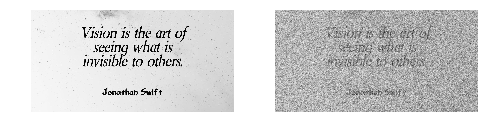
\includegraphics[scale = 0.5]{Trash.png}
\end{center}

\begin{lstlisting}[language=Python]
fig, (ax1,ax2) = plt.subplots(1,2)
im1 = ax1.imshow(A)
im2 = ax2.imshow(An)

ax1.axis('off')
ax2.axis('off')
\end{lstlisting}

\part [2] Plot the first $100$ singular values of $A$ and $\tilde{A}$. ({\em Hint:} Use the \verb|semilogy| plotting function).  
\begin{center}
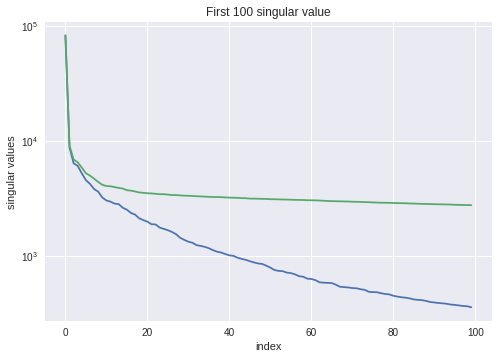
\includegraphics[scale = 0.5]{pp.png}
\end{center}

\begin{lstlisting}[language=Python]
A_U, A_S, A_V = np.linalg.svd(A, full_matrices=False)
An_U, An_S, An_V = np.linalg.svd(An, full_matrices=False)

fig2, ax2 = plt.subplots()
plt.semilogy(np.arange(0,100),A_S[np.arange(0,100)])
plt.semilogy(np.arange(0,100),An_S[np.arange(0,100)])
ax2.set_title('First 100 singular value')
ax2.set_xlabel('index')
ax2.set_ylabel('singular values')
\end{lstlisting}

\part [3] In a single figure with 9 different subplots, plot $A_k$ (the best rank-$k$ approximation to $A$) as images for $k = 5,10,\dots,45$ (use these same values of $k$ for the rest of this problem). 
\begin{center}
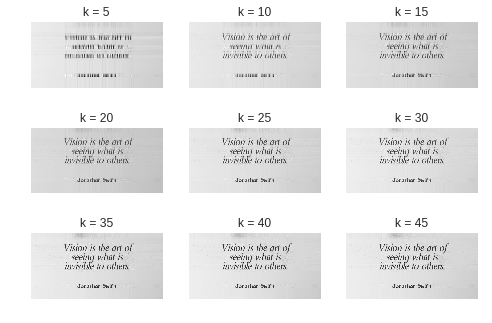
\includegraphics[scale = 0.5]{kill_me.png}
\end{center}

\begin{lstlisting}[language=Python]
ks = [5*x for x in range(1,10)]
error = np.zeros(9)

fig, ((ax1,ax2,ax3),(ax4,ax5,ax6),(ax7,ax8,ax9)) = plt.subplots(3,3)
axes = (ax1,ax2,ax3,ax4,ax5,ax6,ax7,ax8,ax9)
    
for i in range(9):
  k = ks[i]
  ax = axes[i]
  Ek = np.diag(A_S[:k])
  A_k = np.dot(A_U[:,:k],np.dot(Ek, A_V[:k,:]))
  error[i] = np.linalg.norm(A - A_k, 'fro') / np.linalg.norm(A,'fro')

  
  ax.axis('off')
  ax.imshow(A_k)
  ax.set_title('k = %d' % k)
\end{lstlisting}

\pagebreak

\part  [2] As two subplots of the same figure, plot (left panel) the storage cost of the truncated SVD as a function of $k$, (right panel) relative error of $A_k$ (in the Frobenius norm) as a function of $k$. Comment on these two subplots. (Assume that each floating point number requires $1$ unit of storage.)
\begin{center}
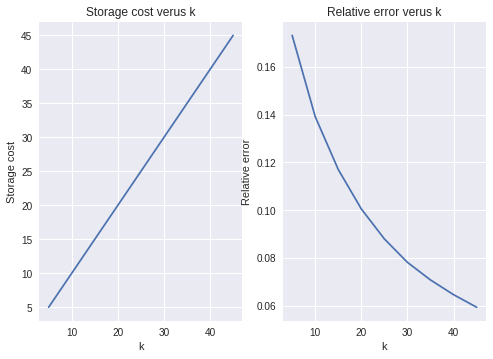
\includegraphics[scale = 0.5]{ded.png}
\end{center}

\begin{lstlisting}[language=Python]
fig, (ax1,ax2) = plt.subplots(1,2)
cost = []

for i in range (9):
  cost.append((ks[i] * (A_k.shape[0] * A_k.shape[1] + 1)/(A_k.shape[0]*A_k.shape[1])))

ax1.plot(ks, cost)
ax2.plot(ks, error)

ax1.set_title('Storage cost verus k')
ax1.set_xlabel('k')
ax1.set_ylabel('Storage cost')

ax2.set_title('Relative error verus k')
ax2.set_xlabel('k')
ax2.set_ylabel('Relative error')
\end{lstlisting}

\part [3] Our proposed algorithm to denoise the image is to use a truncated SVD of the matrix corresponding to the noisy image, i.e., computing $\tilde{A}_k$. In a single figure with 9 different subplots, plot $\tilde{A}_k$ (the best rank-$k$ approximation to $A$) as images for $k = 5,10,\dots,45$. Make sure to label each subplot.
\begin{center}
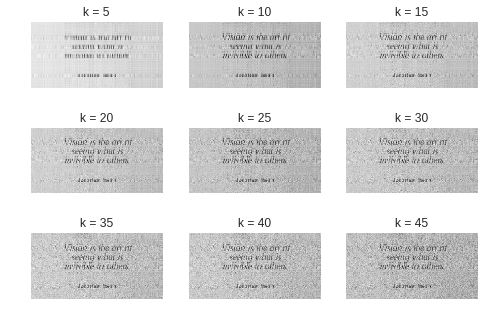
\includegraphics[scale = 0.5]{I_am_in_hell.png}
\end{center}

\begin{lstlisting}[language=Python]
ks = [5*x for x in range(1,10)]
error = np.zeros(9)

fig, ((ax1,ax2,ax3),(ax4,ax5,ax6),(ax7,ax8,ax9)) = plt.subplots(3,3)
axes = (ax1,ax2,ax3,ax4,ax5,ax6,ax7,ax8,ax9)
    
for i in range(9):
  k = ks[i]
  ax = axes[i]
  Ek = np.diag(An_S[:k])
  An_k = np.dot(An_U[:,:k],np.dot(Ek, An_V[:k,:]))
  error[i] = np.linalg.norm(An - An_k, 'fro') / np.linalg.norm(An,'fro')

  
  ax.axis('off')
  ax.imshow(An_k)
  ax.set_title('k = %d' % k)
\end{lstlisting}

\part [2] Plot the relative error of the denoised image $\tilde{A}_k$ (in the Frobenius norm) as a function of the truncation index $k$. For (approximately) what value of $k$ is the minimum attained?
\begin{center}
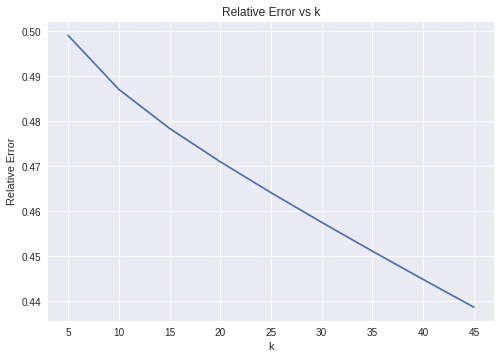
\includegraphics[scale = 0.5]{Hi_satan.png}
\end{center}

\begin{lstlisting}[language=Python]
fig, ax1 = plt.subplots()

ax1.plot(ks, error)

ax1.set_title('Relative Error vs k')
ax1.set_ylabel('Relative Error')
ax1.set_xlabel('k')
\end{lstlisting}

\part  [2 bonus] A result in perturbation analysis (due to Herman Weyl) says
 \[ \max_{1\leq j \leq \min\{m,n\}} |\sigma_j(A+E) - \sigma_j(A)| \leq \|E\|_2.\]
In the context of the noisy images, give an interpretation of the above equation in your words. Based on this formula, can you obtain a lower bound for the amount of noise, measured as $\|E\|_2$? 
\end{parts}
{\em Instructions}: In total, you have to submit $6$ separate plots. Make sure to label each plot/subplot, and label the axes of the singular value and the error plots. 

\question [15] {\em Deblurring} an image. 
\begin{parts}
\part [0] Load the file `deblur.mat'. You will find the variables \verb|A|  (blurring operator, size $4096\times 4096$) and \verb|bn| (blurred and noisy image, size $4096\times 1$), \verb|xtrue| (true image, size $4096\times 1$).
\subsection*{Code}
\begin{lstlisting}[language=Python]
import numpy as np
from scipy.io import loadmat
from matplotlib import pyplot as plt

# save data
dat = loadmat('deblur.mat')
A = dat['A']
bn = dat['bn']
xtrue = dat['xtrue']
\end{lstlisting}

\part [2] In a single figure with 2 subplots, plot the true image,  and the blurry image with noise. Note that you will have to reshape the vectors into $64\times 64$ images. 

\begin{center}
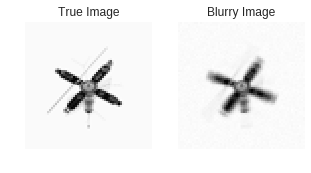
\includegraphics[scale = 0.5]{truevsblurry.png}
\end{center}

\subsection*{Code}
\begin{lstlisting}[language=Python]
import numpy as np
from scipy.io import loadmat
from matplotlib import pyplot as plt

# plot true and blurry image
fig, (ax1,ax2) = plt.subplots(1,2, figsize=(5,10))

# true image
ax1.grid(False)
ax1.axis('off')
ax1.imshow(np.reshape(xtrue,(64,64)))
ax1.set_title('True Image')

# blurry image
ax2.grid(False)
ax2.axis('off')
ax2.imshow(np.reshape(bn,(64,64)))
ax2.set_title('Blurry Image')
\end{lstlisting}

\part [2] Recall the naive solution $x_n = A^{-1}\changes{b_n}$. Plot this solution as an image. (MATLAB users should look up backslash \verb|\|, and Python users should look up \verb|numpy.linalg.solve|. Do not compute the inverse of the matrix!) 

\begin{center}
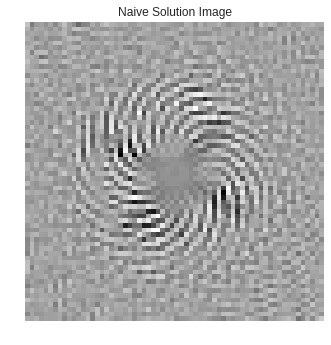
\includegraphics[scale = 0.5]{naive.png}
\end{center}

\subsection*{Code}
\begin{lstlisting}[language=Python]
import numpy as np
from scipy.io import loadmat
from matplotlib import pyplot as plt

# apply naive solution and plot

xn = np.linalg.solve(A,bn)
fig, ax1 = plt.subplots(1,1)
ax1.grid(False)
ax1.axis('off')
ax1.imshow(np.reshape(xn,(64,64)))
ax1.set_title('Naive Solution Image')
\end{lstlisting}

\part [3] Compute the condition number $\kappa_2(A) = \|A\|_2 \|A^{-1}\|_2$ of the matrix $A$. Using perturbation analysis explain why you expect the naive solution to perform poorly (you are given that $\|e\|_2/\|b\|_2 = \changes{0.05}$). 

The condition number is equal to $5039.94$ because it is sooooo large, the error is not well conditioned and very sensitive to perturbation.

\part [3] Implement the truncated SVD formula 
\[ x_k = \sum_{j=1}^k v_j \frac{u_j^\top \changes{b_n}	}{\sigma_j} , \]
for $k = 400,800,\dots,3600$. In a single figure with 9 subplots, plot the reconstructed vectors $x_k$ as images. 

\begin{center}
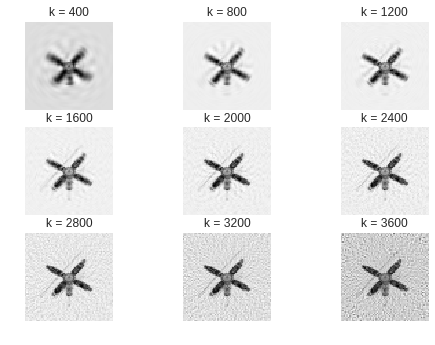
\includegraphics[scale = 0.5]{trunk.png}
\end{center}

\subsection*{Code}
\begin{lstlisting}[language=Python]
import numpy as np
from scipy.io import loadmat
from matplotlib import pyplot as plt

# svd

U, E, VT = np.linalg.svd(A)

# apply truncated svd formula and plot
ks = [400*x for x in range(1,10)]
fig, ((ax1,ax2,ax3),(ax4,ax5,ax6),(ax7,ax8,ax9)) = plt.subplots(3,3)
axes = (ax1,ax2,ax3,ax4,ax5,ax6,ax7,ax8,ax9)

# transpose matrices
UT = np.matrix.transpose(U)
V = np.matrix.transpose(VT)

# save error
error = np.zeros(9)
trueNorm = np.linalg.norm(xtrue, 2)

for i in range(9):
  k = ks[i]
  ax = axes[i]
  Ek = np.diag(1/E[:k]) # just use k singular values
  # apply formula using matrix multiplication
  xk = np.dot(V[:,:k],np.dot(Ek, UT[:k,:]))
  xk = np.matmul(xk, np.reshape(bn,(bn.shape[0],1)))
  error[i] = np.linalg.norm(xtrue - xk, 2) / trueNorm
  # plot image
  ax.grid(False)
  ax.axis('off')
  ax.imshow(np.reshape(xk,(64,64)))
  ax.set_title('k = %d' % k)
\end{lstlisting}
 
\part [3] Plot the relative error in the reconstructed solution as a function of $k$. For (approximately) what value of $k$ is the minimum attained?\\
\\
The minimum is attained at $k=2000$

\begin{center}
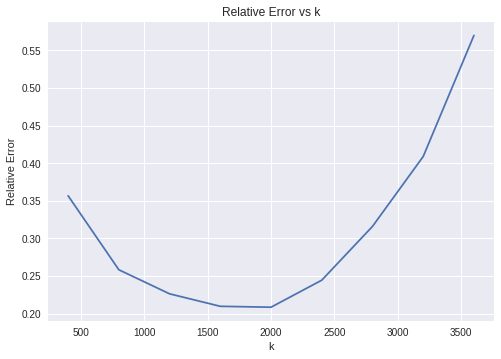
\includegraphics[scale = 0.5]{relvsk.png}
\end{center}

\subsection*{Code}
\begin{lstlisting}[language=Python]
import numpy as np
from scipy.io import loadmat
from matplotlib import pyplot as plt

# plot error
fig, ax1 = plt.subplots(1,1)

ax1.plot(ks, error)
ax1.set_title('Relative Error vs k')
ax1.set_ylabel('Relative Error')
ax1.set_xlabel('k')
\end{lstlisting}
 
\part [2] In your words, explain the behavior of the error as a function of $k$.\\
\\
If $k$ is smaller than 2000 then the truncated image is missing certain details and if it is larger than 2000, noise begins to dominate the reconstruction.

\end{parts}
{\em Instructions}: In total, you have to submit $4$ separate plots. Make sure to label each plot/subplot, and label the axes of the error plots.
\end{questions}


\end{document}


